\documentclass{article}
\usepackage[utf8]{inputenc}
\usepackage[brazil]{babel}

% Necessário para o GEOGEBRA
\usepackage{pgfplots}
\pgfplotsset{compat=1.15}
\usepackage{mathrsfs}
\usetikzlibrary{arrows}

% Necessário para matemática
\usepackage{amsfonts}
\usepackage{amsmath}
\usepackage{amssymb}
\usepackage{amsthm}

% Pacote extra para matemática \sfrac{}
\usepackage{xfrac}


\usepackage{hyperref}
\pagestyle{empty}

\hypersetup{
    colorlinks=true,
    linkcolor=blue,
    filecolor=magenta,      
    urlcolor=cyan,
    pdftitle={Monitoria 2},
    pdfpagemode=FullScreen,
    }

\title{Monitoria 2}
\author{Eduardo Adame Salles}
\date{\today}


\begin{document}

\maketitle

\section{Introduction}

% Importar GEOGEBRA
\definecolor{uuuuuu}{rgb}{0.26666666666666666,0.26666666666666666,0.26666666666666666}
\definecolor{zzttqq}{rgb}{0.6,0.2,0.1}
\definecolor{ududff}{rgb}{0.30196078431372547,0.30196078431372547,1.}

\begin{tikzpicture}[line cap=round,line join=round,>=triangle 45,x=1.0cm,y=1.0cm]
\begin{axis}[
x=1.0cm,y=1.0cm,
axis lines=middle,
ymajorgrids=true,
xmajorgrids=true,
xmin=-5,
xmax=5,
ymin=-4.2,
ymax=5,
xtick={-10.0,-8.0,...,12.0},
ytick={-6.0,-4.0,...,6.0},]
\clip(-11.566352666963397,-6.164582699666525) rectangle (12.992631551171927,6.47795526306048);
\fill[line width=2.pt,color=zzttqq,fill=zzttqq,fill opacity=0.10000000149011612] (-1.36197164673073,-0.24054192016981435) -- (0.34543144351879096,1.6121720713775345) -- (-1.5072825480285574,3.3195751616270552) -- (-3.2146856382780786,1.466861170079707) -- cycle;
\fill[line width=2.pt,color=zzttqq,fill=zzttqq,fill opacity=0.10000000149011612] (0.34543144351879096,1.6121720713775345) -- (-3.2146856382780786,1.466861170079707) -- (-4.176623438949835,-1.9639149173058599) -- (-1.2110166130314335,-3.9389402458026934) -- (1.583767003326588,-1.7287969400700953) -- cycle;
\fill[line width=2.pt,color=zzttqq,fill=zzttqq,fill opacity=0.10000000149011612] (-1.36197164673073,-0.24054192016981435) -- (1.583767003326588,-1.7287969400700953) -- (4.345502982898606,0.07816005383907965) -- (4.161500312413306,3.3733720676485373) -- (1.2157616623559893,4.861627087548819) -- (-1.5459743172160296,3.054670093639645) -- cycle;
\draw [line width=2.pt,color=zzttqq] (-1.36197164673073,-0.24054192016981435)-- (0.34543144351879096,1.6121720713775345);
\draw [line width=2.pt,color=zzttqq] (0.34543144351879096,1.6121720713775345)-- (-1.5072825480285574,3.3195751616270552);
\draw [line width=2.pt,color=zzttqq] (-1.5072825480285574,3.3195751616270552)-- (-3.2146856382780786,1.466861170079707);
\draw [line width=2.pt,color=zzttqq] (-3.2146856382780786,1.466861170079707)-- (-1.36197164673073,-0.24054192016981435);
\draw [line width=2.pt,color=zzttqq] (0.34543144351879096,1.6121720713775345)-- (-3.2146856382780786,1.466861170079707);
\draw [line width=2.pt,color=zzttqq] (-3.2146856382780786,1.466861170079707)-- (-4.176623438949835,-1.9639149173058599);
\draw [line width=2.pt,color=zzttqq] (-4.176623438949835,-1.9639149173058599)-- (-1.2110166130314335,-3.9389402458026934);
\draw [line width=2.pt,color=zzttqq] (-1.2110166130314335,-3.9389402458026934)-- (1.583767003326588,-1.7287969400700953);
\draw [line width=2.pt,color=zzttqq] (1.583767003326588,-1.7287969400700953)-- (0.34543144351879096,1.6121720713775345);
\draw [line width=2.pt,color=zzttqq] (-1.36197164673073,-0.24054192016981435)-- (1.583767003326588,-1.7287969400700953);
\draw [line width=2.pt,color=zzttqq] (1.583767003326588,-1.7287969400700953)-- (4.345502982898606,0.07816005383907965);
\draw [line width=2.pt,color=zzttqq] (4.345502982898606,0.07816005383907965)-- (4.161500312413306,3.3733720676485373);
\draw [line width=2.pt,color=zzttqq] (4.161500312413306,3.3733720676485373)-- (1.2157616623559893,4.861627087548819);
\draw [line width=2.pt,color=zzttqq] (1.2157616623559893,4.861627087548819)-- (-1.5459743172160296,3.054670093639645);
\draw [line width=2.pt,color=zzttqq] (-1.5459743172160296,3.054670093639645)-- (-1.36197164673073,-0.24054192016981435);
\begin{scriptsize}
\draw [fill=ududff] (-1.36197164673073,-0.24054192016981435) circle (2.5pt);
\draw[color=ududff] (-1.2088680184454557,0.14600846247170157) node {$A$};
\draw [fill=ududff] (0.34543144351879096,1.6121720713775345) circle (2.5pt);
\draw[color=ududff] (0.49958305759874094,2.0039490076697577) node {$B$};
\draw[color=zzttqq] (-1.67512379994903,1.726325707812577) node {\tiny Quadrado};
\draw [fill=uuuuuu] (-1.5072825480285574,3.3195751616270552) circle (2.5pt);
\draw[color=uuuuuu] (-1.3583574875993227,3.7124000837139475) node {$C$};
\draw [fill=uuuuuu] (-3.2146856382780786,1.466861170079707) circle (2.5pt);
\draw[color=uuuuuu] (-3.066808563643519,1.8544595385158913) node {$D$};
\draw[color=zzttqq] (-1.0807341877421408,-0.7082170755503934) node {Pentágono};
\draw [fill=uuuuuu] (-4.176623438949835,-1.9639149173058599) circle (2.5pt);
\draw[color=uuuuuu] (-4.02781229391838,-1.5624426135724883) node {$E$};
\draw [fill=uuuuuu] (-1.2110166130314335,-3.9389402458026934) circle (2.5pt);
\draw[color=uuuuuu] (-1.0593785492915884,-3.5485169894738586) node {$F$};
\draw [fill=uuuuuu] (1.583767003326588,-1.7287969400700953) circle (2.5pt);
\draw[color=uuuuuu] (1.7382100877307833,-1.327530590616412) node {$G$};
\draw[color=zzttqq] (1.6527875339285736,1.769036984713682) node {\tiny Hexágono};
\draw [fill=uuuuuu] (4.345502982898606,0.07816005383907965) circle (2.5pt);
\draw[color=uuuuuu] (4.49308744785205,0.46634303922998716) node {$H$};
\draw [fill=uuuuuu] (4.161500312413306,3.3733720676485373) circle (2.5pt);
\draw[color=uuuuuu] (4.3008867017970775,3.7764669990656046) node {$I$};
\draw [fill=uuuuuu] (1.2157616623559893,4.861627087548819) circle (2.5pt);
\draw[color=uuuuuu] (1.3751642340713917,5.250006052153719) node {$J$};
\draw [fill=uuuuuu] (-1.5459743172160296,3.054670093639645) circle (2.5pt);
\draw[color=uuuuuu] (-1.4010687645004276,3.456132422307319) node {$K$};
\end{scriptsize}
\end{axis}
\end{tikzpicture}

% Ambiente Matemático
\section{Ambiente Matemático}

\subsection{Em linha}
$ax +b =0$\\
\( ax + b = 0 \)

Lorem ipsum dolor it amet $x=4$.

\subsection{Omae wa}

\subsection{Destacado}
\label{ss:dest}

$$ ax + b = 0  $$

\[ ax + b = 0 \]

Eu tenho \$10,00.

\begin{itemize}
    \item Índice: $x_1$ ou $x_{12}$
    \item Expoente: $x^2$ ou $x^{zky}$
    \item Os dois: $x_j^k$ e $x_{y^z}^k$
    \item Fração: $\frac{1}{2}$ ou $\dfrac{1}{2}$ e $\sfrac{1}{2}$
    \item Radical: $\sqrt{b^2-4ac}$ ou $\sqrt[n]{x}$
    \item Letras Gregas: $\alpha$, $\phi$, $\rho$, $\pi$, $\beta$, $\gamma$, $\omega$, $\lambda$, $\chi$, $\delta$, $\epsilon$, $\varepsilon$, $\varphi$, $\kappa$, $\sigma$
    \item Especiais: $$\sum_{i=0}^{\infty} a_i$$, $$\int_{a}^{b} f(x)\ dx$$, $\prod$, $\nabla$, $\partial$, $\mathbb{R}$, $\mathbb{Q}$, $\mathcal{P}$
    
    $a \cdot b = ab$, $a \times b$, $\hat{x}$, $\vec{x}$, $\bar{x}$
    
    $\underbrace{a \div b}_{\frac{a}{b}}$
    $\overbrace{a \div b}^{\frac{a}{b}}$ $\blacksquare$
        
    $\text{Eduardo} + Adame = \text{Eduardo Adame}$ 
    
    $\sin{30}$, $\cos{40}$, $\ln{a}$, $\log{a}$, $\to$, $$\lim_{x \to 0} x$$, $\forall$, $\therefore$, $\implies$, $\iff$, $\in$, $\cup$, $\cap$, $\not\in$
    
\end{itemize}

    \begin{align*}
        ax^2 + bx + c &= 0\\
        ax^2 + bx &= -c\\
        x^2 + \frac{b}{a}x &= -\frac{c}{a}
    \end{align*}
    
    $$
    \begin{bmatrix}
    1 & 0\\
    0 & 1
    \end{bmatrix}
    $$
    
    
    \begin{equation}
        e^{i\pi} + 1 = 0
        \label{eq:eul}
    \end{equation}
    
    \begin{equation}
        \sin{\theta}^2 + \cos{\theta}^2 = 1
        \label{eq:id}
    \end{equation}
    
    
    Lorem ipsum dolor sit amet. A equação \eqref{eq:eul} é muito bonita. Como você viu na subseção \ref{ss:dest}
    %\begin{proof}
    %Seja $a_n$ uma sequência.
    %\end{proof}
    
    \subsection{Referências}
    
    O livro ~\cite{stewart2020} é ótimo. Acesse \cite{salles}.
    

    \bibliography{references}{}
    \bibliographystyle{apalike}
    
    \subsection{Figuras}
    
    \begin{figure}[!h]
        \centering
        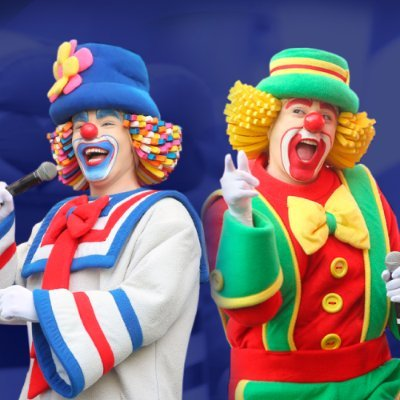
\includegraphics[width=.5\textwidth]{patati.jpg}
        \caption{Legenda maneira}
        \label{fig:massa}
    \end{figure}
    
    A imagem \ref{fig:massa} retrata dois dos maiores brasileiros de todos os tempos.

\end{document}

